% Drawing 144/04-9 -- folder 144, batch 04, archive page 80 (PDF page 81).
% Transcription: Dans la marge gauche, une sphère : $P_\omega$ en haut, $P_{\omega'}$ en bas, deux demi-méridiens en pointillé $\lambda$ passant par $Q_{\omega' a}$ et $Q_a$ sur l'équateur, avec $R_s$ entre eux.
% Kind: sphere with two dotted half-meridians, Q_{omega' a}, R_s, Q_a. Method 2 (schematic redraw from the facsimile). Status: ok.
% Notes: Pencil sphere and equator; two dotted half-meridians lambda from P_omega to P_omega' through Q_{omega' a} and Q_a, with R_s between them.
% Coordinates: 1 unit = 1 mm = 1/100 of the crop width (bbox in page fractions: [0.1, 0.415, 0.28, 0.56]).
% Redrawn by Claude (claude-opus-5-5), issue #73, 2026-11-07; not checked by a human; not compiled (no TeX in the session).
% Rights: reproduces part of the work -- behind RENDER_TRANSCRIPTS, never published by itself.
\documentclass[tikz,border=3pt]{standalone}
\usepackage{amsmath,amssymb}
\usetikzlibrary{patterns,arrows.meta}
\tikzset{pencil/.style={black!45}, struck/.style={black!35}, mark/.style={circle,draw,inner sep=1.3pt}, pt/.style={circle,fill,inner sep=0.9pt}, opt/.style={circle,draw,fill=white,inner sep=1.1pt}}
\begin{document}
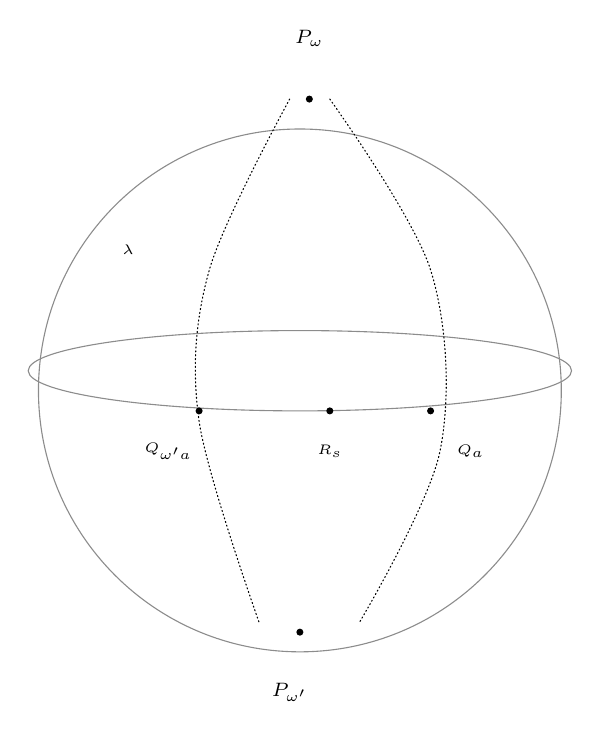
\begin{tikzpicture}[x=1mm,y=1mm,line cap=round,line join=round,font=\scriptsize]
\draw[pencil] (45.1,-62.5) circle[radius=33.2];
\draw[pencil] (45.1,-60) ellipse[x radius=34.5, y radius=5.1];
\draw[densely dotted] plot[smooth, tension=0.55] coordinates {(43.8,-25.5) (33.6,-47.2) (32.3,-66.4) (39.9,-91.9)};
\draw[densely dotted] plot[smooth, tension=0.55] coordinates {(48.9,-25.5) (61.7,-47.2) (62.9,-70.2) (52.7,-91.9)};
\node[pt] at (46.3,-25.5) {};
\node[pt] at (45.1,-93.2) {};
\node[pt] at (32.3,-65.1) {};
\node[pt] at (48.9,-65.1) {};
\node[pt] at (61.7,-65.1) {};
\node[inner sep=1pt] at (46.3,-17.8) {\scriptsize $P_\omega$};
\node[inner sep=1pt] at (43.8,-100.9) {\scriptsize $P_{\omega'}$};
\node[inner sep=1pt] at (28.4,-70.2) {\tiny $Q_{\omega' a}$};
\node[inner sep=1pt] at (48.9,-70.2) {\tiny $R_s$};
\node[inner sep=1pt] at (66.8,-70.2) {\tiny $Q_a$};
\node[inner sep=1pt] at (23.3,-44.6) {\tiny $\lambda$};
\end{tikzpicture}
\end{document}
